\pdfoutput=1
\documentclass[11pt]{article}
\usepackage{authblk}
\usepackage[review]{acl2023}
\usepackage{times}
\usepackage{graphicx}
\usepackage{latexsym}
\usepackage{array}
\usepackage{booktabs}
\setlength{\heavyrulewidth}{1.5pt}
\setlength{\abovetopsep}{4pt}
\usepackage{pgfplots}
\usepackage{algorithm}
\usepackage{algpseudocode}
\usepackage{graphicx}
\usepackage[T1]{fontenc}
\usepackage[utf8]{inputenc}
\usepackage{microtype}
\usepackage{xcolor}
\usepackage{soul}
\usepackage{subcaption}
\usepackage{tikz}
\usepackage{pgfplots}
\usepackage{adjustbox}
\usepackage{times}
\usepackage{xcolor}
\usepackage{graphicx}
\usepackage{latexsym}
\usepackage{array}
\usepackage{booktabs}
\setlength{\heavyrulewidth}{1.5pt}
\setlength{\abovetopsep}{4pt}
\usepackage{pgfplots}
\usepackage{algorithm}
\usepackage{algpseudocode}
\usepackage{graphicx}
\usepackage[T1]{fontenc}
\usepackage[utf8]{inputenc}
\usepackage{microtype}
\usepackage{xcolor}
\usepackage{soul}
\usepackage{fullpage}
\usepackage{enumitem}
\usepackage{pgfplots}
\usepackage{algorithm}
\usepackage{algpseudocode}
\usepackage{graphicx}
\usepackage{placeins}
\usepackage{tabularx}
\usepackage{makecell}
\usepackage{booktabs}       % professional-quality tables
\usepackage{array}          % tables with fixed lengths - enables using "m" to center content of non-multirow cells
\usepackage{colortbl}
\newcolumntype{P}[1]{>{\centering\arraybackslash}p{#1}}
\newcolumntype{M}[1]{>{\centering\arraybackslash}m{#1}}
\newcommand{\greyrule}{\arrayrulecolor{black!30}\midrule\arrayrulecolor{black}}
\usepackage{amsmath}
\usepackage{mathtools}
\title{Quick Dense Retrievers Consume KALE: Post Training Kullback–Leibler Alignment of Embeddings for Asymmetrical dual encoders}
\author[1]{Daniel Campos \thanks{~~~Corresponding author: dcampos3@illinois.edu}}
\author[2]{Alessandro Magnani}
\author[1]{ChengXiang Zhai}
\affil[1]{Department of Computer Science, the University of Illinois Urbana-Champaign}
\affil[2]{Walmart Labs}
\begin{document}
\maketitle
\begin{abstract}
In this paper, we consider the problem of improving the inference latency of language model-based dense retrieval systems by introducing structural compression and model size asymmetry between the context and query encoders. First, we investigate the impact of pre and post-training compression on the MSMARCO, Natural Questions, TriviaQA, SQUAD, and SCIFACT, finding that asymmetry in the dual-encoders in dense retrieval can lead to improved inference efficiency. Knowing this, we introduce \emph{Kullback–Leibler Alignment of Embeddings} (KALE), an efficient and accurate method for increasing the inference efficiency of dense retrieval methods by pruning and aligning the query encoder after training. Specifically, KALE extends traditional Knowledge Distillation after bi-encoder training, allowing for effective query encoder compression without full retraining or index generation. Using KALE and asymmetric training, we can generate models which exceed the performance of DistilBERT despite having 3x faster inference. 
\end{abstract}
\section{Introduction}
\begin{figure}[!htb]
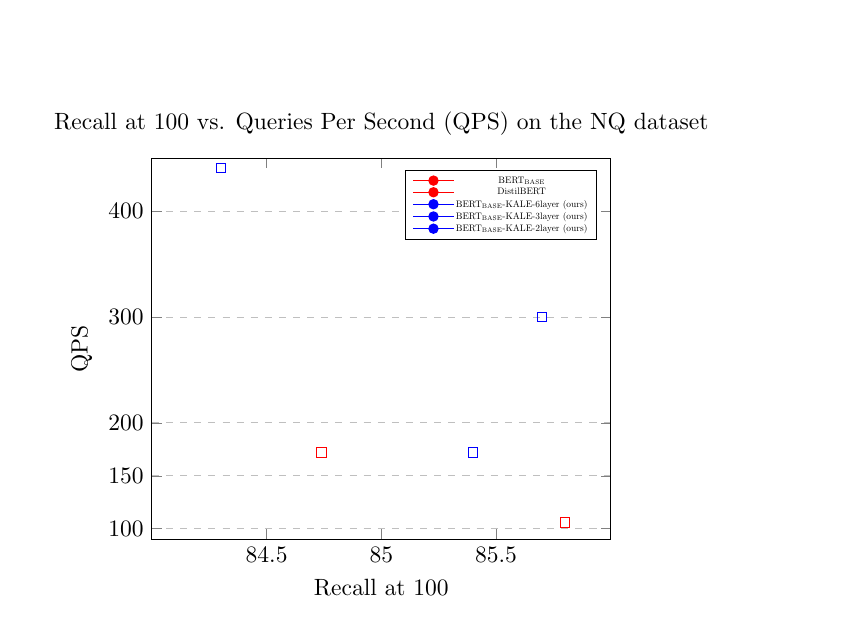
\begin{tikzpicture}
\scalebox{0.85}{
\begin{axis}[
    title={Recall at 100 vs. Queries Per Second (QPS) on the NQ dataset},
    xlabel={Recall at 100},
    ylabel={QPS},
    xmin=84, xmax=86,
    ymin=90 , ymax=450,
    xtick={84.5, 85, 85.5},
    ytick={100, 150, 200, 300,400},
    legend pos=north east,
    ymajorgrids=true,
    grid style=dashed,
    legend style={nodes={scale=0.4, transform shape}}, 
    legend image post style={mark=*}
]
\addplot[
    color=red,
    mark=square,
    ]
    coordinates {
    (85.8,106)
    };

\addplot[
    color=red,
    mark=square,
    ]
    coordinates {
    (84.74,172)
    };
\addplot[
    color=blue,
    mark=square,
    ]
    coordinates {
    (85.4,172)
    };
\addplot[
    color=blue,
    mark=square,
    ]
    coordinates {
    (85.7,300)
    };
\addplot[
    color=blue,
    mark=square,
    ]
    coordinates {
    (84.3,441)
    };

\legend{BERT\textsubscript{BASE}, DistilBERT, BERT\textsubscript{BASE}-KALE-6layer (ours),BERT\textsubscript{BASE}-KALE-3layer (ours), BERT\textsubscript{BASE}-KALE-2layer (ours) }
 \end{axis}}
\end{tikzpicture}
    \centering
    \caption{Using KALE and asymmetric training on the lead to when measuring QPS vs. Recall at 100 on the NQ dataset. Using Asymmetry and KALE, it is possible to 3x QPS with no loss in accuracy and 4.5x with 1\% loss in performance. We calculate QPS as the mean number of queries per second with a batch size of 1 and a max sequence length of 32 on a T4 GPU}
    \label{fig:speed}
\end{figure}
The application of sequence-to-sequence language models has become an important tool for natural language processing tasks such as machine translation \cite{Sutskever2014SequenceTS}, audio transcription \cite{Radford2022RobustSR}, and abstractive summarization \cite{Raffel2020ExploringTL}. Sequence-to-sequence models effectively turn each of these aforementioned tasks into two-step problems: extraction and generation, and heavily condition the generation on the input. \\
Besides ensuring on-topic responses sequence to sequence models have the added benefit of being able to map inputs to targets with varying lengths and modalities in ways encoder or decoder-only systems cannot. \\
When used for abstractive summarization, sequence-to-sequence modeling has two steps, extraction using the encoder and generation using the decoder, which usually involves repeated execution until an end-of-sequence token is emitted. While the cost of encoder execution is essentially fixed on the batch size, the cost of decoder execution can be highly variable and difficult to predict. Despite the broad study of sequence-to-sequence models and how they compress research which studies the role of model symmetry as applied to inference efficiency and model accuracy is lacking. \\
Recent advances in scaling language models have led to a wide study on \textit{scaling laws} as applied to language model performance \cite{Kaplan2020ScalingLF}, training data size \cite{Hoffmann2022TrainingCL}, machine translation \cite{Henighan2020ScalingLF}, and even reinforcement learning \cite{Neumann2022ScalingLF}. \\
We build on this work and study the impact of scaling on abstractive summarization and what role model asymmetry has in it.
This asymmetry can manifest in various ways, such as the number of layers and hidden units in the encoder and decoder and the type of attention mechanisms used. \\
In this paper, we explore the role of asymmetry in the number of layers in encoder-decoder language modeling for summarization and its impact on the performance of these models. As shown in figure \ref{fig:speed}, the symmetry of pruning drives the impact on accuracy and inference speedups for sequence-to-sequence models. Pruning the encoder portion of the network leads to virtually no improvement in inference speed at the expense of accuracy. Pruning the decoder provides speedup with minor losses in accuracy. 
The following research questions drive our work: 
\begin{itemize}
    \item What scaling laws can be observed in abstractive summarization?
    \item What impact does encoder-decoder asymmetry have on abstractive summarization accuracy? 
    \item What impact does encoder-decoder asymmetry have on abstractive summarization inference efficiency?
    \item What is asymmetries impact on accuracy and inference efficiency does scale have in encoder-decoder models for abstractive summarization? 
\end{itemize}
It is in answering these questions that we deliver the following contributions: 
\begin{itemize}
\item We present the first robust study on scaling laws applied to the compression of sequence-to-sequence modeling. 
\item We demonstrate that the asymmetric inference cost of sequence-to-sequence models leads to asymmetric pruning for optimal inference efficient compression.
\item We empirically demonstrate on a wide variety of benchmarks how Asymmetric Compression can lead to a 2.7x inference speedup with no loss in accuracy on the XSUM dataset.
\end{itemize}
\section{Related Work}
\textbf{Bi-Encoders}, commonly called dual-encoders or dense retrievers, decompose ranking by leveraging the inner product of query and document representations to produce a relevance score for query document pairs. Since their document representations are query invariant, they can be pre-computed and loaded into an Approximate Nearest Neighbor (ANN) such as FAISS \cite{johnson2019billion}. The $k$ closest documents can be found for each query with minimal latency at run time. Since bi-encoders leverage LLM such as BERT \cite{Devlin2019BERTPO}, they are often limited to ranking short passages of text and are commonly referred to as Dense Passage Retrievers (DPR) \cite{Karpukhin2020DensePR}. Driven by their efficiency in deployment and relevance performance, DPR-based models have rapidly become the building blocks for systems doing product search \cite{Magnani2022SemanticRA}, open domain question answering \cite{Karpukhin2020DensePR} and customer support \cite{Mesquita2022DenseTR}.\\
Recent work has heavily focused on improving the relevance of DPR models by improving the negative sampling using methods like ANCE \cite{Xiong2021ApproximateNN} and in-batch negatives \cite{Lin2021InBatchNF}. While effective DPR models are brittle to shifts in the domain, minor variations can cause a complete collapse in relevance. Li et al. '2022 introduced methods for improving such performance by having a single query encoder leverage multiple document encoders to transfer between domains \cite{Li2022AnEA}. While effective, such a method carries a high computational load as multiple indexes must be maintained and updated. \\
\textbf{Data Augmentation} (DA) is a popular approach for improving how well models perform on new or noisy data. In data augmentation, training is extended by augmenting the training data with modifications or perturbations which match the desired model behavior. DA is extremely common in computer vision where training data is commonly rotated, blurred, cropped, or zoomed-in/out \cite{Mikoajczyk2018DataAF} \cite{Zhong2020RandomED}. \\
DA has become increasingly more popular in NLP and has been used to improve model performance \cite{Jiao2020TinyBERTDB}, simulate large-scale training data when it is not available \cite{Li2020ADD}, and mitigate bias \cite{Lu2020GenderBI} in existing datasets. A detailed survey on DA approaches for NLP has been complied by Feng et al. 21' \cite{Feng2021ASO}.\\
\textbf{Contrastive Learning} builds on the notion of a contrastive loss \cite{Chopra2005LearningAS}, which seeks to create clusters in the embedding space such that examples with a shared class are far from other classes but close to each other. Much like learning that queries with noise have a shared intent, Schroff et al. 15' leverage contrastive learning to recognize faces despite different angles and perspectives \cite{Schroff2015FaceNetAU} by using a triplet loss. This approach is a natural fit for the world of search as relevance is at its core clustering relevant items close together and far from irrelevant items. Recently, contrastive learning has become a method for learning relevance at the corpora scale \cite{Xiong2021ApproximateNN} and improving DPR on noisy queries, \cite{Sidiropoulos2022AnalysingTR} \cite{Chen2022TowardsRD}
\section{Method}
\subsection{Generating Noisy Queries}
\label{sec:making-noise}
While previous work has studied the impact of minor variations to queries, such as typos and misspellings, query noise is much more diverse. Seeking to expand this understanding, we explore the impact of query alterations that evaluate surface, syntactic, and semantic alterations. To apply noise to a query, we either edit a query to introduce a specific type of noise or rewrite the query to simulate similarly worded intents. Each query that is altered has a notion of its anchor, either a character, word or a group of words, which is selected where noise is applied. To achieve this for each query, a character or word index is randomly selected. Then, noise is applied to the left, right, or at the noising index (replacing the existing index) with equal probability. Example alterations are in table \ref{tab:query-noise}. \\
To study the impact of surface-level alterations, we introduce noise in queries by simulating misspellings and typos by swapping, eliminating, or shuffling characters in a query. To understand how models respond to typos or character omissions, we delete a character (DC), inject a random character (RCS), or simulate a keyboard-based typo by injecting a character close to its neighbor on a keyboard (KCS). We swap the indexed word with another word in the query to understand how systems may work when faced with natural shifts in keyword queries. \\
To study syntactic alterations, we introduce noise that alters the syntax of the query introducing lemmas, stems, synonyms, and determiners using tools from the NLTK toolkit \cite{bird2009natural}. Synonyms are introduced using NLTK's interface with WordNet \cite{Fellbaum2000WordNetA}, and exact synonyms for a single word are introduced.  Determiners, affixes that occur with nouns and commonly are not discriminative for search, are introduced similarly to typos to the left or right of noun phrases. Lemma's return words to their canonical root while stemming reduced word inflection using the Porter-stemmer. We select up to five words per query to attempt stemming/lemmatization, but many queries do not have any words which can be stemmed or lemmatized versions and, as a result, are un-noised. \\
Exploring semantically similar queries, we leverage paraphrasing, back-translation, and synonyms. To paraphrase, we rewrite queries using a T5 \cite{Raffel2020ExploringTL} sequence-to-sequence model, which has been fine-tuned on the PAWS \cite{Zhang2019PAWSPA} dataset. For back-translation, we use OpenNMT's \cite{klein-etal-2017-opennmt} to translate queries from English to another language and then back to English after exploring performance using German, French, Italian, and Spanish to find the German to have the best quality and use only those. It is worth noting that these semantic noising methods are the most likely to alter the true query intent, as seen by the 'hallucinations' in table \ref{tab:query-noise} paraphrase alteration. \\
Using the aforementioned noising approaches, we noise the queries on the MSMARCO \cite{Campos2016MSMA} \footnote{https://huggingface.co/datasets/spacemanidol/msmarco-passage-query-variation} \footnote{https://huggingface.co/datasets/spacemanidol/rewrite-noisy-queries}, Natural Questions \footnote{https://huggingface.co/datasets/spacemanidol/wikipedia-nq-query-variation} \footnote{https://huggingface.co/datasets/spacemanidol/nq-noising} \cite{Kwiatkowski2019NaturalQA}, and the Trivia QA \cite{Joshi2017TriviaQAAL} \footnote{https://huggingface.co/datasets/spacemanidol/wikipedia-trivia-query-variation} Passage Ranking datasets. \\
\subsection{Baseline Performance}
\begin{figure}[!htb]
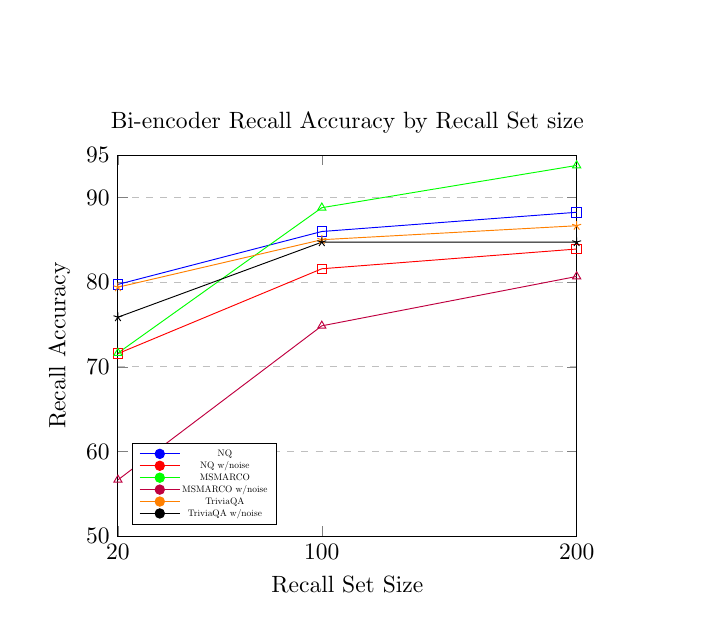
\begin{tikzpicture}
\scalebox{0.85}{
\begin{axis}[
    title={Bi-encoder Recall Accuracy by Recall Set size},
    xlabel={Recall Set Size},
    ylabel={Recall Accuracy},
    xmin=20, xmax=200,
    ymin=50 , ymax=95,
    xtick={20, 100, 200},
    ytick={50, 60, 70, 80, 90, 95},
    legend pos=south west,
    ymajorgrids=true,
    grid style=dashed,
    legend style={nodes={scale=0.4, transform shape}}, 
    legend image post style={mark=*}
]
\addplot[
    color=blue,
    mark=square,
    ]
    coordinates {
    (20, 79.73) (100, 85.98) (200, 88.25)
    };
\addplot[
    color=red,
    mark=square,
    ]
    coordinates {
    (20, 71.56) (100,81.58) (200, 83.91)
    };
\addplot[
    color=green,
    mark=triangle,
    ]
    coordinates {
    (20, 71.63) (100, 88.79) (200, 93.78)
    };
    
\addplot[
    color=purple,
    mark=triangle,
    ]
    coordinates {
    (20, 56.65) (100, 74.84) (200, 80.67)
    };
\addplot[
    color=orange,
    mark=star,
    ]
    coordinates {
    (20, 79.40) (100,85.01) (200, 86.66)
    };
\addplot[
    color=black,
    mark=star,
    ]
    coordinates {
    (20, 75.86) (100, 84.72) (200, 84.72)
    };
\legend{NQ, NQ w/noise, MSMARCO, MSMARCO w/noise, TriviaQA, TriviaQA w/noise}
 \end{axis}}
\end{tikzpicture}
    \centering
    \caption{Bi-encoder recall accuracy on noisy and non-noisy queries with variations of recall set size and datasets. }
    \label{fig:baseline-impact-query-noise}
\end{figure}
In production workloads, bi-encoders are most commonly used for early retrieval, where the sets they produce are then reranked using a cross-encoder. Given cross-encoder are more robust to typos \cite{Sidiropoulos2022AnalysingTR}, our work focuses exclusively on evaluating the impact of noise on the retrieval accuracy of bi-encoders. \\
To do so, we train  a series of task-specific bi-encoders leveraging the open-source bi-encoder-focused library Tevatron \cite{Gao2022TevatronAE} with task-specific training parameters found in \ref{tab:capot-bi-encoder-hy} on the widely used and studied MSMARCO \cite{Campos2016MSMA}, Natural Questions (NQ) \cite{Kwiatkowski2019NaturalQA} and TriviaQA \cite{Joshi2017TriviaQAAL} passage retrieval datasets. \\
For contextual representations, each encoder uses  a pre-trained BERT \cite{Devlin2019BERTPO} model for its initialization, and we use separate models for the query and document models. Representations are taken from the unaltered 768-dimension vectors based on the last hidden representation of the CLS token. \\
For each dataset, we train each model using 5 different random seeds with fixed optimal hyperparameters, generate seed and task-specific indexes and evaluate the retrieval impact of queries with noise and unaltered routes. We evaluate the impact on retrieval by measuring the impact on retrieval accuracy at $k$ with a $k={20,100,200}$.  \\
As shown in figure \ref{fig:baseline-impact-query-noise} on the impact of averaged noise, our experimental results align with prior research. There is a wide variation of impact as the long, trivia-inspired queries of Trivia QA see minor losses in accuracy compared to the real-world web search queries of MSMARCO, up to 12\% the impact. Besides the impact of query type, we also notice the large role recall set size plays on the relative degradation in retrieval accuracy. Across tasks and datasets, increasing the recall set from 20 to 200 decreases the impact on accuracy by about 50\%. \\ 
Focusing on the impacts of individual types of noise shown in \ref{sec:full-noise-impact}, we see that queries with surface alteration, such as typos, see the largest loss. Despite featuring real-world search engine queries with noise, on MSMARCO, there is nearly a 30\% loss in retrieval accuracy for queries with typos, dropping from 71\% to 41\%. On all datasets, queries with character-level alterations see a 50\% average higher loss in accuracy than other alterations. This large gap can be attributed to the vocabulary construction method of BERT and BERT-like models, where a minor alteration to a single character can produce large variations in tokenization.\\
In the absence of model optimization, data augmentation, or post-training optimization, the clearest way to make dense retrieval robust to noise is to expand the recall set and allow cross-encoders to re-rank the expanded results.\\
\section{KL Alignment of Embeddings}
\begin{table}[!htb]
    \centering
    \caption{Impact of structural pruning with and without KALE on Accuracy at 100 across various datasets. }
    \tiny
    \scalebox{0.8}{
    \begin{tabular}{|l|l|l|l|l|l|l|}
    \hline
        Layers & KALE & NQ & TriviaQA & MSMARCO & SCIFACT & SQUAD \\ \hline
        12 & N/A & 85.84\% & 85.84\% & 88.77\% & 90.70\% & 77.16\% \\ \hline
        9 & N & 79.97\% & 79.97\% & 82.01\% & 71.07\% & 71.38\% \\ \hline
        9 & Y & 84.90\% & 84.90\% & 86.16\% & 84.87\% & 73.54\% \\ \hline
        6 & N & 68.20\% & 68.20\% & 72.68\% & 22.98\% & 59.97\% \\ \hline
        6 & Y & 83.68\% & 83.68\% & 84.68\% & 85.13\% & 69.87\% \\ \hline
        3 & N & 43.88\% & 43.88\% & 11.39\% & 40.80\% & 34.42\% \\ \hline
        3 & Y & 81.14\% & 81.14\% & 82.11\% & 82.57\% & 64.37\% \\ \hline
        2 & N & 46.90\% & 46.90\% & 31.46\% & 42.66\% & 37.01\% \\ \hline
        2 & Y & 81.94\% & 81.94\% & 81.96\% & 82.57\% & 63.72\% \\ \hline
        1 & N & 12.22\% & 12.22\% & 0.00\% & 3.17\% & 11.66\% \\ \hline
        1 & Y & 71.33\% & 71.33\% & 54.36\% & 66.83\% & 51.39\% \\ \hline
    \end{tabular}}
    \label{tab:kale-at-20}
\end{table}
While training asymmetric models can improve latency, it requires novel training regimes and experimentation, and existing workloads need to regenerate their entire index to take advantage of any inference speedups. Generation of the passage index can take longer than model training \cite{Karpukhin2020DensePR}, which makes regenerating a new index and retraining a model to meet changing latency requirements an inefficient experimentation pathway. \\Moreover, coupling asymmetry into training makes generating query encoder variants more difficult, as each encoder requires its own index and document encoder. \\
Motivated by this bottleneck, we introduce \textbf{K}ullback-Leibler \textbf{Al}lingment of \textbf{E}mbeddings (KALE), a simple method of improving bi-encoder latency by aligning the embeddings of compressed models. KALE is applied after model training and leverages large batch sizes to make compression \textbf{computationally inexpensive} and \textbf{independent of training}. A single V100 GPU KALE can produce a compressed query encoder in less than 5 minutes.  \\
First, a bi-encoder model trains with separate query and document encoders. When training is complete, the document encoder, $e_{document}$, is frozen, and using the query encoder, $e_{q}$, a structurally pruned copy, $e_{q'}$, is made. Then, using a sample of queries, the $e_{q'}$ model is fine-tuned to minimize the KL divergence of their query representations as shown in equation \ref{kale-eq:1}. \\
\begin{equation}\label{kale-eq:1} 
    \displaystyle D_{\text{KL}}(e_{q'} \parallel e_{q} )= \sum _{x\in {\mathcal {X}}}e_{q'}(x)\log \left({\frac {e_{q'}(x)}{e_{q}(x)}}\right).
\end{equation}
We explored the use of various distance functions such as cosine similarity, Manhattan distance, and the KL divergence but found little sensitivity in any metric besides KL divergence. We believe this is due to us freezing the document representations, and as a result, cosine distance allows the query embeddings to \textit{drift} more than probability distribution matching methods. To explore this further, we experiment with tuning the temperature for the KL divergence and add a loss scaling factor but find a temperature of one and a scaling factor of ten to be most optimal. \\
Additionally, we explored using a contrastive loss with random negative and hard negatives mined from the trained encoder but found no positive impact for either method. We leave further exploration of training objective improvement for future work.
\begin{figure*}
    \centering
    \begin{subfigure}[b]{0.35\textwidth}
   \begin{adjustbox}{width=\linewidth}
      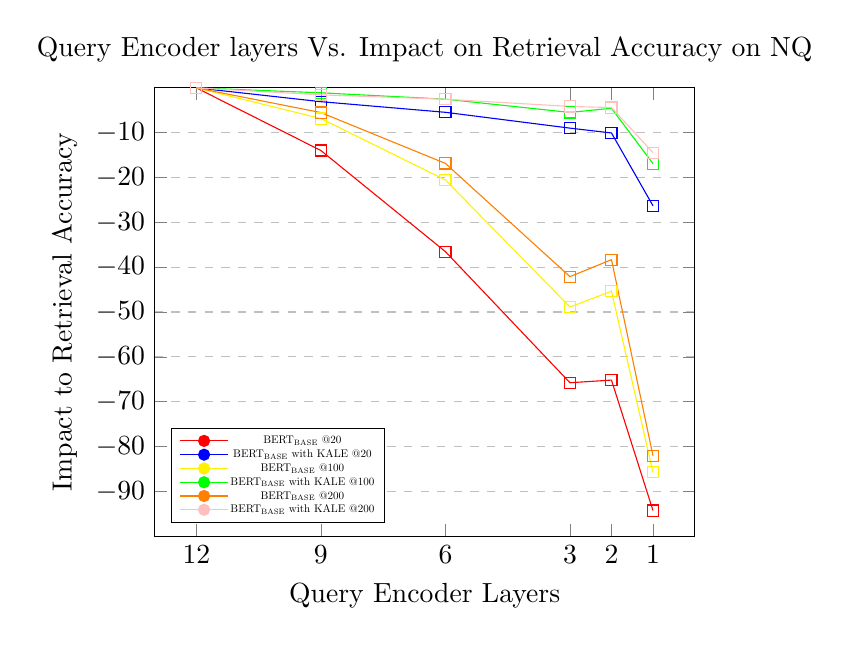
\begin{tikzpicture}
\begin{axis}[
    title={Query Encoder layers Vs. Impact on Retrieval Accuracy on NQ},
    xlabel={Query Encoder Layers},
    ylabel={Impact to Retrieval Accuracy},
    xmin=0, xmax=13,
    x dir=reverse,
    ymin=-100 , ymax=0,
    xtick={1,2,3,6,9,12},
    ytick={-10,-20,-30,-40, -50,-60,-70,-80,-90},
    legend pos=south west,
    ymajorgrids=true,
    grid style=dashed,
    legend style={nodes={scale=0.4, transform shape}}, 
    legend image post style={mark=*}
]
\addplot[
    color=red,
    mark=square,
    ]
    coordinates {
    (12, 0) (9, -13.97) (6,-36.53) (3,-65.77) (2, -65.18) (1, -94.28)
    };

\addplot[
    color=blue,
    mark=square,
    ]
    coordinates {
    (12, 0) (9, -3.08) (6, -5.45) (3,-8.98) (2,-10.06) (1, -26.30)

    };
\addplot[
    color=yellow,
    mark=square,
    ]
    coordinates {
    (12, 0) (9, -6.84) (6,-20.55) (3,-48.88) (2, -45.36) (1, -85.76)
    };

\addplot[
    color=green,
    mark=square,
    ]
    coordinates {
    (12, 0) (9, -1.10) (6, -2.52) (3,-5.48) (2,-4.54) (1, -16.90)

    };
\addplot[
    color=orange,
    mark=square,
    ]
    coordinates {
    (12, 0) (9, -5.51) (6,-16.85) (3,-42.11) (2, -38.32) (1, -82.05)
    };

\addplot[
    color=pink,
    mark=square,
    ]
    coordinates {
    (12, 0) (9, -1.56) (6, -2.53) (3,-4.14) (2,-4.39) (1, -14.44)

    };
\legend{BERT\textsubscript{BASE} @20, BERT\textsubscript{BASE} with KALE @20,BERT\textsubscript{BASE} @100, BERT\textsubscript{BASE} with KALE @100,BERT\textsubscript{BASE} @200, BERT\textsubscript{BASE} with KALE @200}
 \end{axis}
\end{tikzpicture}
 \end{adjustbox} 
\end{subfigure} 
    \begin{subfigure}[b]{0.382\textwidth}
   \begin{adjustbox}{width=\linewidth} 
      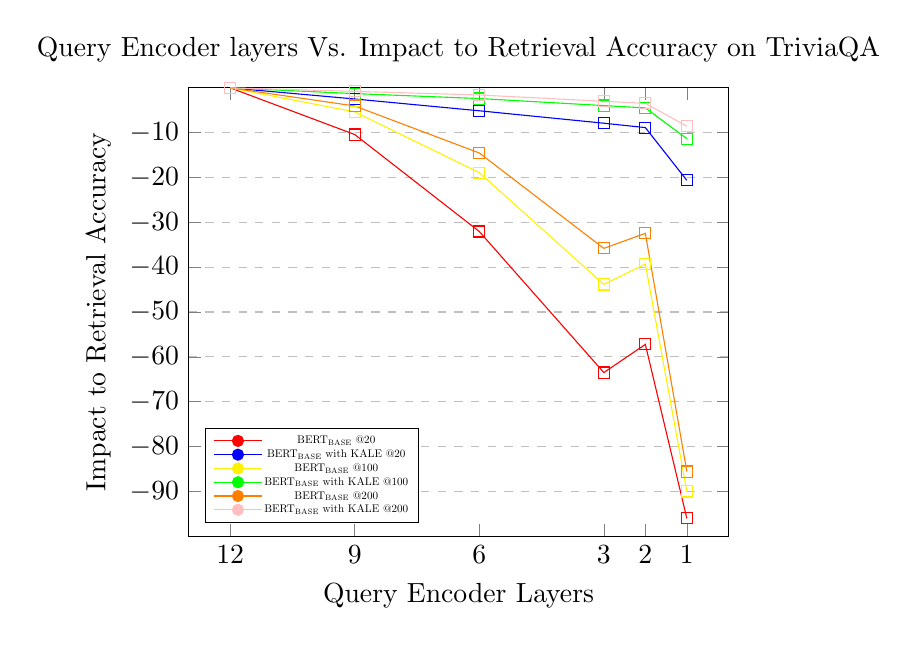
\begin{tikzpicture}
        \begin{axis}[
            title={Query Encoder layers Vs. Impact to Retrieval Accuracy on TriviaQA},
            xlabel={Query Encoder Layers},
            ylabel={Impact to Retrieval Accuracy},
            xmin=0, xmax=13,
            x dir=reverse,
            ymin=-100 , ymax=0,
            xtick={1,2,3,6,9,12},
            ytick={-10,-20,-30,-40, -50,-60,-70,-80,-90},
            legend pos=south west,
            ymajorgrids=true,
            grid style=dashed,
            legend style={nodes={scale=0.4, transform shape}}, 
            legend image post style={mark=*}
        ]
        \addplot[
            color=red,
            mark=square,
            ]
            coordinates {
            (12, 0) (9, -10.41) (6,-32.04) (3,-63.5) (2, -57.22) (1, -96.03)
            };
        
        \addplot[
            color=blue,
            mark=square,
            ]
            coordinates {
            (12, 0) (9, -2.48) (6, -5.11) (3,-7.88) (2,-8.86) (1, -20.63)
        
            };
        \addplot[
            color=yellow,
            mark=square,
            ]
            coordinates {
            (12, 0) (9, -5.35) (6,-18.91) (3,-43.84) (2, -39.29) (1, -90.02)
            };
        
        \addplot[
            color=green,
            mark=square,
            ]
            coordinates {
            (12, 0) (9, -1.28) (6,-2.38) (3,-3.95) (2, -4.47) (1, -11.33)
            };
        
        \addplot[
            color=orange,
            mark=square,
            ]
            coordinates {
            (12, 0) (9, -4.04) (6, -14.52) (3,-35.8) (2,-32.45) (1, -85.58)
        
            };
        \addplot[
            color=pink,
            mark=square,
            ]
            coordinates {
            (12, 0) (9, -0.78) (6,-1.59) (3,-2.99) (2, -3.45) (1, -8.54)
            };
        \legend{BERT\textsubscript{BASE} @20, BERT\textsubscript{BASE} with KALE @20,BERT\textsubscript{BASE} @100, BERT\textsubscript{BASE} with KALE @100,BERT\textsubscript{BASE} @200, BERT\textsubscript{BASE} with KALE @200}
         \end{axis}
        \end{tikzpicture}
         \end{adjustbox}       
    \end{subfigure}
    \\
    \begin{subfigure}[b]{0.4\textwidth}
       \begin{adjustbox}{width=\linewidth} % rescale box
          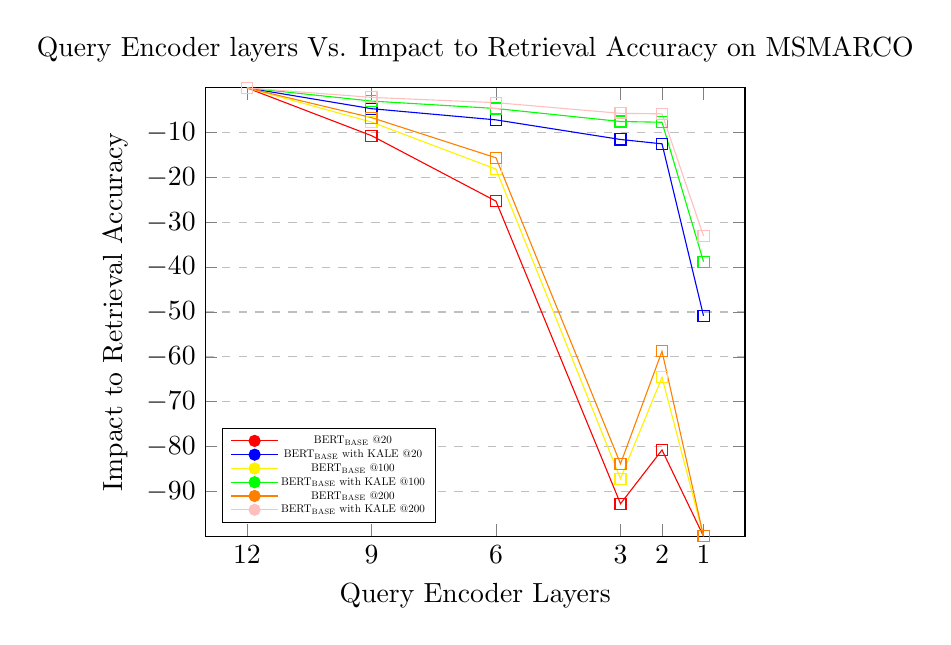
\begin{tikzpicture}
            \begin{axis}[
                title={Query Encoder layers Vs. Impact to Retrieval Accuracy on MSMARCO},
                xlabel={Query Encoder Layers},
                ylabel={Impact to Retrieval Accuracy},
                xmin=0, xmax=13,
                x dir=reverse,
                ymin=-100 , ymax=0,
                xtick={1,2,3,6,9,12},
                ytick={-10,-20,-30,-40, -50,-60,-70,-80,-90},
                legend pos=south west,
                ymajorgrids=true,
                grid style=dashed,
                legend style={nodes={scale=0.4, transform shape}}, 
                legend image post style={mark=*}
            ]
            \addplot[
                color=red,
                mark=square,
                ]
                coordinates {
                (12, 0) (9, -10.65) (6,-25.27) (3,-92.76) (2, -80.77) (1, -100)
                };
            
            \addplot[
                color=blue,
                mark=square,
                ]
                coordinates {
                (12, 0) (9, -4.64) (6, -7.14) (3,-11.51) (2,-12.48) (1, -50.84)
            
                };
            \addplot[
                color=yellow,
                mark=square,
                ]
                coordinates {
                (12, 0) (9, -7.62) (6,-18.12) (3,-87.17) (2, -64.56) (1, -100)
                };
            
            \addplot[
                color=green,
                mark=square,
                ]
                coordinates {
                (12, 0) (9, -2.94) (6, -4.6) (3,-7.5) (2,-7.67) (1, -38.77)
            
                };
            \addplot[
                color=orange,
                mark=square,
                ]
                coordinates {
                (12, 0) (9, -6.63) (6,-15.6) (3,-83.85) (2, -58.75) (1, -100)
                };
            
            \addplot[
                color=pink,
                mark=square,
                ]
                coordinates {
                (12, 0) (9, -2.12) (6, -3.3) (3,-5.68) (2,-5.79) (1, -33.05)
            
                };
            \legend{BERT\textsubscript{BASE} @20, BERT\textsubscript{BASE} with KALE @20,BERT\textsubscript{BASE} @100, BERT\textsubscript{BASE} with KALE @100,BERT\textsubscript{BASE} @200, BERT\textsubscript{BASE} with KALE @200}
             \end{axis}
            \end{tikzpicture}
        \end{adjustbox}       
    \end{subfigure} \\ 
    \begin{subfigure}[b]{0.38\textwidth}
       \begin{adjustbox}{width=\linewidth} % rescale box
          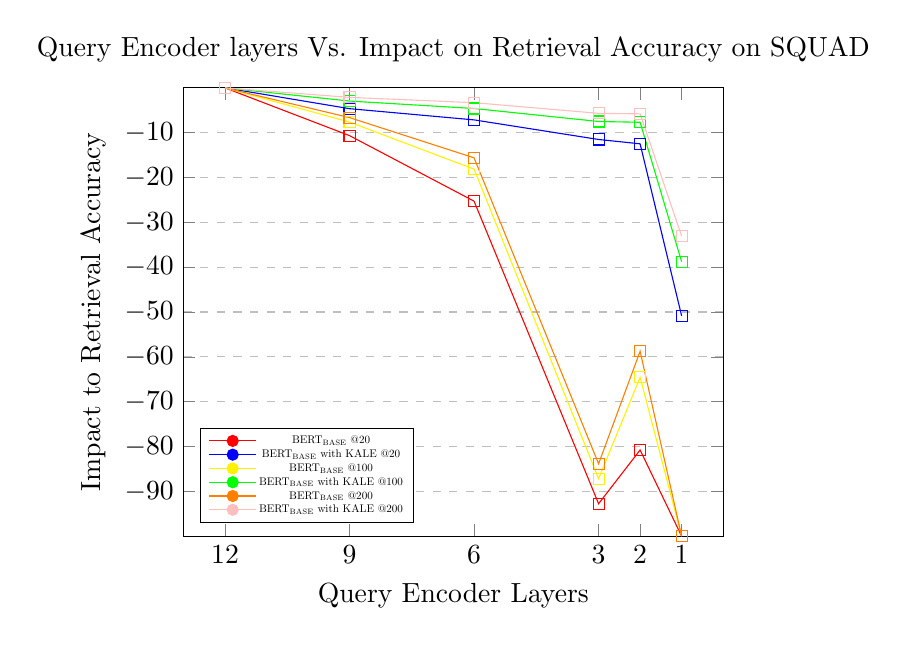
\begin{tikzpicture}
            \begin{axis}[
                title={Query Encoder layers Vs. Impact on Retrieval Accuracy on SQUAD},
                xlabel={Query Encoder Layers},
                ylabel={Impact to Retrieval Accuracy},
                xmin=0, xmax=13,
                x dir=reverse,
                ymin=-100 , ymax=0,
                xtick={1,2,3,6,9,12},
                ytick={-10,-20,-30,-40, -50,-60,-70,-80,-90},
                legend pos=south west,
                ymajorgrids=true,
                grid style=dashed,
                legend style={nodes={scale=0.4, transform shape}}, 
                legend image post style={mark=*}
            ]
            \addplot[
                color=red,
                mark=square,
                ]
                coordinates {
                (12, 0) (9, -10.65) (6,-25.27) (3,-92.76) (2, -80.77) (1, -100)
                };
            
            \addplot[
                color=blue,
                mark=square,
                ]
                coordinates {
                (12, 0) (9, -4.64) (6, -7.14) (3,-11.51) (2,-12.48) (1, -50.84)
            
                };
            \addplot[
                color=yellow,
                mark=square,
                ]
                coordinates {
                (12, 0) (9, -7.62) (6,-18.12) (3,-87.17) (2, -64.56) (1, -100)
                };
            
            \addplot[
                color=green,
                mark=square,
                ]
                coordinates {
                (12, 0) (9, -2.94) (6, -4.6) (3,-7.5) (2,-7.67) (1, -38.77)
            
                };
            \addplot[
                color=orange,
                mark=square,
                ]
                coordinates {
                (12, 0) (9, -6.63) (6,-15.6) (3,-83.85) (2, -58.75) (1, -100)
                };
            
            \addplot[
                color=pink,
                mark=square,
                ]
                coordinates {
                (12, 0) (9, -2.12) (6, -3.3) (3,-5.68) (2,-5.79) (1, -33.05)
            
                };
            \legend{BERT\textsubscript{BASE} @20, BERT\textsubscript{BASE} with KALE @20,BERT\textsubscript{BASE} @100, BERT\textsubscript{BASE} with KALE @100,BERT\textsubscript{BASE} @200, BERT\textsubscript{BASE} with KALE @200}
             \end{axis}
            \end{tikzpicture}
        \end{adjustbox}
    \end{subfigure} 
    \begin{subfigure}[b]{0.4\textwidth}
       \begin{adjustbox}{width=\linewidth} % rescale box
          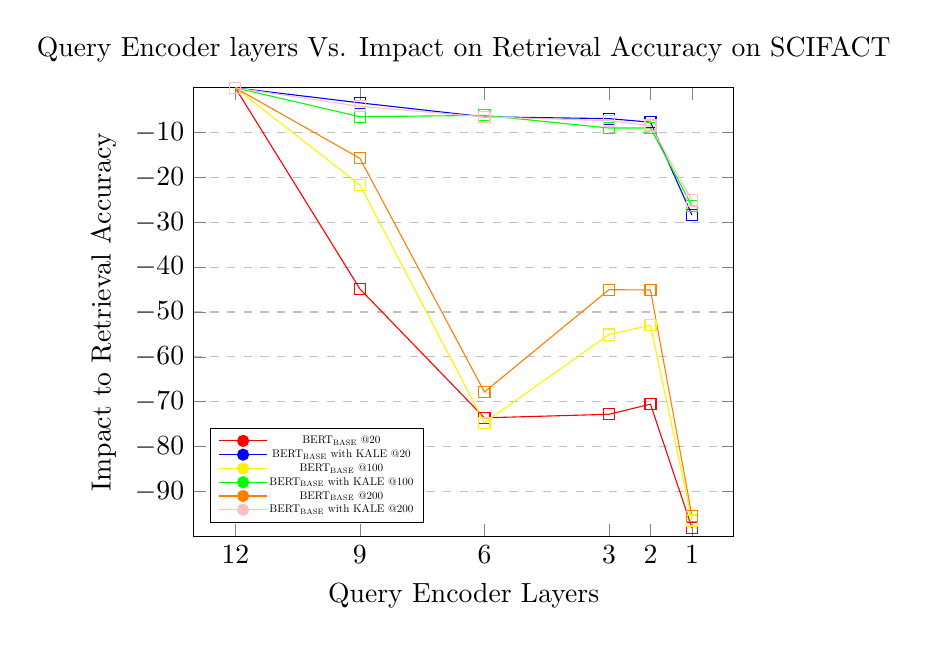
\begin{tikzpicture}
            \begin{axis}[
                title={Query Encoder layers Vs. Impact on Retrieval Accuracy on SCIFACT},
                xlabel={Query Encoder Layers},
                ylabel={Impact to Retrieval Accuracy},
                xmin=0, xmax=13,
                x dir=reverse,
                ymin=-100 , ymax=0,
                xtick={1,2,3,6,9,12},
                ytick={-10,-20,-30,-40, -50,-60,-70,-80,-90},
                legend pos=south west,
                ymajorgrids=true,
                grid style=dashed,
                legend style={nodes={scale=0.4, transform shape}}, 
                legend image post style={mark=*}
            ]
            \addplot[
                color=red,
                mark=square,
                ]
                coordinates {
                (12, 0) (9, -44.85) (6,-73.60) (3,-72.81) (2, -70.55) (1, -98.18)
                };
            
            \addplot[
                color=blue,
                mark=square,
                ]
                coordinates {
                (12, 0) (9, -3.34) (6,-6.45) (3,-6.86) (2, -7.66) (1, -28.38)
                };
            \addplot[
                color=yellow,
                mark=square,
                ]
                coordinates {
                (12, 0) (9, -21.64) (6,-74.66) (3,-55.02) (2, -52.95) (1, -96.50)
                };
            
            \addplot[
                color=green,
                mark=square,
                ]
                coordinates {
                (12, 0) (9, -6.43) (6,-6.14) (3,-8.96) (2, -8.96) (1, -26.32)
                };
            \addplot[
                color=orange,
                mark=square,
                ]
                coordinates {
                (12, 0) (9, -15.72) (6,-67.83) (3,-45.01) (2, -45.09) (1, -95.49)
                };
            
            \addplot[
                color=pink,
                mark=square,
                ]
                coordinates {
                (12, 0) (9, -4.13) (6,-6.47) (3,-7.33) (2, -8.39) (1, -25.11)
                };
            \legend{BERT\textsubscript{BASE} @20, BERT\textsubscript{BASE} with KALE @20,BERT\textsubscript{BASE} @100, BERT\textsubscript{BASE} with KALE @100,BERT\textsubscript{BASE} @200, BERT\textsubscript{BASE} with KALE @200}
             \end{axis}
            \end{tikzpicture}
        \end{adjustbox}
    \end{subfigure}
    \caption{Impact of structural pruning with and without KALE on the NQ, MSMARCO, TriviaQA, SciFACT, and SQuAD Passage Retrieval dataset with the recall set sizes of 20,100, and 200. Across datasets, we see a consistent trend where KALE is effective but most effective when the network is heavily pruned and recall set sizes are small. When the model is pruned to 2 or 1 layer with a recall set size of 20, the difference between using KALE or not can be up to 10 times the loss in recall accuracy}
    \label{fig:kale-not}
\end{figure*}
\subsection{Experimental Results}
We evaluate the effectiveness of KALE by taking uncompressed BERT\textsubscript{BASE} models and pruning them with and without KALE on a variety of well-established passage retrieval benchmarks. First, models are trained, and indexes are generated using un-optimized BERT\textsubscript{BASE} models. Next, the document encoders are frozen, and the query encoders are structurally pruned to have 9,6,3,2 or 1 transformer layer. Finally, query encoders are aligned using KALE, and we compare the performance of compressed models by comparing the impact on retrieval accuracy at 20,100, and 200. \\
To aid reproducibility, each model is trained using the Tevatron \cite{Gao2022TevatronAE} \footnote{https://github.com/texttron/tevatron} library, which makes use of hugginface's transformers to provide a simple interface for exploring neural ranking models. Our experiments focus on the plain BERT\textsubscript{BASE}-uncased 12-layer transformer model. While never more capable models exist, the unaltered BERT model is widely used in production workloads, which our experiments seek to emulate. \\
Our work aims not to produce the highest possible retrieval accuracy for a dense encoder. Instead, our goal is to find the role of asymmetry in bi-encoder models. As a result, we leverage the well-established parameters in all of our experiments without using an advanced methodology like contrastive or curriculum learning. \\
There are fewer parameters for using KALE, and we deliberately do not optimize on anything but the loss between $e_{q}$ and $e_{q'}$. In general, higher degrees of pruning require longer training with smaller batches. \\ 
\textbf{Datasets} We use a wide variety of standard dense retrieval benchmarks, including MSMARCO V1.1 \footnote{https://huggingface.co/datasets/Tevatron/msmarco-passage} \cite{Campos2016MSMA}, NQ Passage Ranking \footnote{https://huggingface.co/datasets/Tevatron/wikipedia-nq} \cite{Kwiatkowski2019NaturalQA}, SciFact Passage Ranking \footnote{https://huggingface.co/datasets/Tevatron/scifact} \cite{Wadden2020FactOF}, TriviaQA passage Ranking \footnote{https://huggingface.co/datasets/Tevatron/wikipedia-trivia} \cite{Joshi2017TriviaQAAL}, and SQUAD Passage Ranking \footnote{https://huggingface.co/datasets/Tevatron/wikipedia-squad} \cite{Rajpurkar2016SQuAD10}. \\
For each dataset, we evaluate performance by measuring the recall accuracy with retrieval depths of 20,100, and 200. Additionally, for the MSMARCO dataset, we also report MRR@10; for Scifact, we also report NDCG @10 and RR@10. \\
\textbf{Computational Experiments}
Our experimentation on fine-tuning our compressed models uses a 16 GB V100 GPU. Experiments in bi-encoder model training leverage 1 V100 for the MSMARCO and 4 for each other experiment. Due to the vast number of models and datasets we train on, each experiment happens with the same fixed seed.  

\textbf{CAPOT and typos} When queries have typos, CAPOT is a computationally efficient method of improving performance as the relative gap between unaltered and aligned is greatest on alterations like character deletion, keyboard character replacement, and random character replacement. We attribute this impact to the relative importance of our alignment dataset's character level alterations. Three out of the 10 methods focus on learning alignments based around minor character shifts, and as a result, the performance optimizes there to the detriment of other forms of noise. CAPOT is much less effective in improving the relevance of minor syntactic shifts such as lemmatization or stemming leading to marginal improvements over the unaltered baselines. We attribute this to the already smaller gap on syntactically altered queries, which on datasets such as TriviaQA have less than 2\% impact.\\
\textbf{CAPOT and Retrieval Set Depth} demonstrates that CAPOT, like DA, sees the highest impact when the recall set size is small. On the NQ the gap between CAPOT and the baseline at 20 is nearly 10\% which narrows to ~3\% at 200.  \\
\textbf{Limitations of contrastive alignment} While effective, contrastive alignment has a non-negligible impact on the retrieval accuracy of unaltered queries. As shown in table \ref{tab:capot-nq-20} on non-noisy queries the use of data augmentation incurs no loss in accuracy yet CAPOT incurs ~2.5\%. This is a fundamental issue because the alignment of embeddings causes minor variations in representations that have actual implications on retrieval accuracy. We believe that the use of larger datasets could such as the web search logs used by the Generic Intent Representation of query vectors \cite{Zhang2019GenericIR} could improve this.\\
\textbf{Poly Encoding} using alignment-based optimization we believe leads to novel retrieval methods which allow for fixed index, constrained optimizations tailored to specific types of noise or deficiencies in retrieval. Novel forms of noise-optimized encoders can be deployed in parallel without additional index generation. Given the prevalence of bi-encoders as candidate set generation tools, CAPOT, unlike Data Augmentation, can generate many targeted query encoder variants which share a document representation. As shown in figure \ref{fig:fig2}, instead of seeking a single query encoder that learns all surface and semantic forms of query representations, alignment approaches can be used to create many encoders which are tuned to various goals. 
\label{app:poly-encoder}
\begin{figure}[htb!]
    \centering
    \scalebox{0.22}{
    \includegraphics{figure2.png}}
    \caption{Proposed poly-encoder architecture using noise-targeted query encoders optimized with CAPOT}
    \label{fig:fig2}
\end{figure}
\bibliographystyle{acl_natbib}
\bibliography{anthology,custom}
\appendix
\section{Introducing and Transferring Sparsity for efficient inference}
\label{app:sparsity}
\section{Robust and Efficient Semantic Retrieval}
\label{app:retrieval}

\section{Scaling Multi-Lingual Classification and Abstractive Summarization to Web-Scale workloads}
\label{app:scaling-workload}

\section{Publications}
\begin{itemize}
\item \href{https://arxiv.org/abs/2203.07259}{The Optimal BERT Surgeon: Scalable and Accurate Second-Order Pruning for Large Language Models} - Eldar Kurtic, \textbf{Daniel Campos}, Tuan Nguyen, Elias Frantar, Mark Kurtz, Benjamin Fineran, Michael Goin, Dan Alistarh - \href{https://2022.emnlp.org/}{EMNLP 2022}
\item \href{https://arxiv.org/abs/2205.12452}{Sparse*BERT: Sparse Models Generalize To New tasks and Domains} - \textbf{Daniel Campos}, Alexandre Marques, Tuan Nguyen, Mark Kurtz, ChengXiang Zhai - \href{https://www.sparseneural.net/}{Sparsity in Neural Networks Workshop at ICML 2022}
\item \href{https://arxiv.org/abs/2303.17612}{oBERTa: Improving Sparse Transfer Learning via improved initialization, distillation, and pruning regimes} - \textbf{Daniel Campos}, Alexandre Marques, Mark Kurtz, ChengXiang Zhai 
\item \href{https://arxiv.org/abs/2304.00114}{Dense Sparse Retrieval: Using Sparse Language Models for Inference Efficient Dense Retrieval} - \textbf{Daniel Campos}, ChengXiang Zhai
\item \href{https://arxiv.org/abs/2304.03401}{Noise-Robust Dense Retrieval via Contrastive Alignment Post Training} - \textbf{Daniel Campos}, Alessandro Magnani, ChengXiang Zhai
\item \href{https://arxiv.org/abs/2304.01016}{Quick Dense Retrievers Consume KALE: Post Training Kullback Leibler Alignment of Embeddings for Asymmetrical dual encoders} - \textbf{Daniel Campos}, Alessandro Magnani, ChengXiang Zhai
\item \href{https://arxiv.org/abs/2211.15927}{Compressing Cross-Lingual Multi-task Models at Qualtrics} - \textbf{Daniel Campos}, Daniel Perry, Samir Joshi, Yashmeet Gambhir, Wei Du, Zhengzheng Xing, and Aaron Colak - \href{https://aaai.org/Conferences/AAAI-23/iaai-23-call/}{The Thirty-Fifth Annual Conference on Innovative Applications of Artificial Intelligence (IAAI-23)}
\item \href{https://arxiv.org/abs/2304.02721}{To Asymmetry and Beyond: Structured Pruning of Sequence to Sequence Models for Improved Inference Efficiency} - \textbf{Daniel Campos}, ChengXiang Zhai
\end{itemize}
\end{document}